%This work is licensed under the Creative Commons License Attribution 4.0 International (CC-BY 4.0)
%https://creativecommons.org/licenses/by/4.0/legalcode
\documentclass[rgb]{standalone}
\usepackage{tkz-euclide}
\definecolor{myorange}{hsb}{0.0833, 1, 0.8}
\definecolor{mygreen}{hsb}{0.3333, 1, 0.8}
\definecolor{myblue}{hsb}{0.5833, 1, 0.8}
\definecolor{mymagenta}{hsb}{0.8333, 1, 0.8}
\begin{document}
	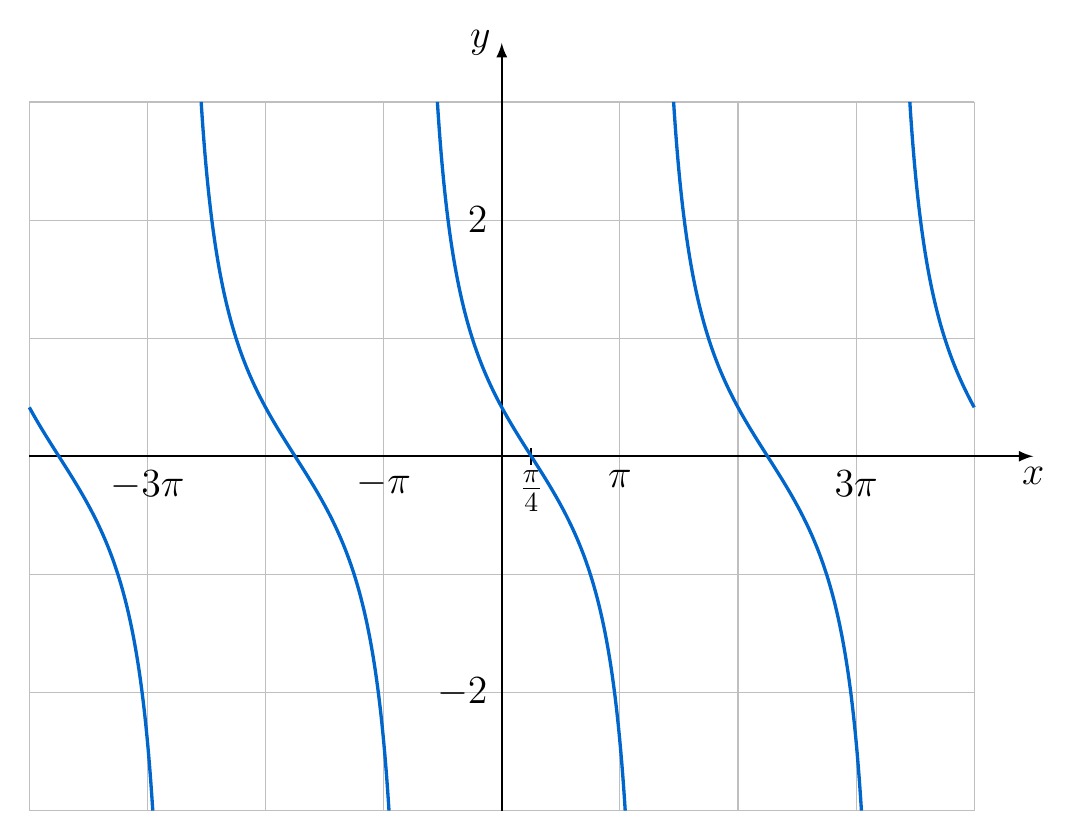
\begin{tikzpicture}[scale=1.5, font=\Large]
		% Coordinate system
		\tkzInit[xmin=-4,xmax=4,ymin=-3,ymax=3]
		\tkzGrid[color=lightgray]
		\tkzDrawX[thick]
		\tkzDrawY[thick] 
		\draw[thick] (0.25,-0.07) -- (0.25,0.07);
		\draw[very thick,domain={135}:{360+2*atan(-1/3)}, smooth, samples=500, variable=\x,myblue] plot ({-4.75+\x/180}, {1/tan(0.5*\x)});
		\draw[very thick,domain={0-2*atan(-1/3)}:{360+2*atan(-1/3)}, smooth, samples=500, variable=\x,myblue] plot ({-2.75+\x/180}, {1/tan(0.5*\x)});
		\draw[very thick,domain={0-2*atan(-1/3)}:{360+2*atan(-1/3)}, smooth, samples=500, variable=\x,myblue] plot ({-0.75+\x/180}, {1/tan(0.5*\x)});
		\draw[very thick,domain={0-2*atan(-1/3)}:{360+2*atan(-1/3)}, smooth, samples=500, variable=\x,myblue] plot ({1.25+\x/180}, {1/tan(0.5*\x)});
		\draw[very thick,domain={0-2*atan(-1/3)}:{135}, smooth, samples=500, variable=\x,myblue] plot ({3.25+\x/180}, {1/tan(0.5*\x)});
		\node[below=0.5mm] at (0.25,0){$\frac{\pi}{4}$};
		\node[below=0.5mm] at (1,0){$\pi$};
		\node[below=0.5mm] at (3,0){$3\pi$}; 
		\node[below=0.5mm] at (-1,0){$-\pi$}; 
		\node[below=0.5mm] at (-3,0){$-3\pi$};
		\node[left=0.5mm] at (0,2){$2$}; 
		\node[left=0.5mm] at (0,-2){$-2$};
	\end{tikzpicture}	
\end{document}